\documentclass[12pt,a4paper]{article}
\usepackage{graphicx}
\usepackage{url}
\usepackage[utf8]{inputenc}

\begin{document}

\begin{titlepage}

\center{\Huge{The Black Box}}
\center{\large{Perception in the 19th century}}
\vspace{1cm}

\begin{figure}[h]
	\centering
	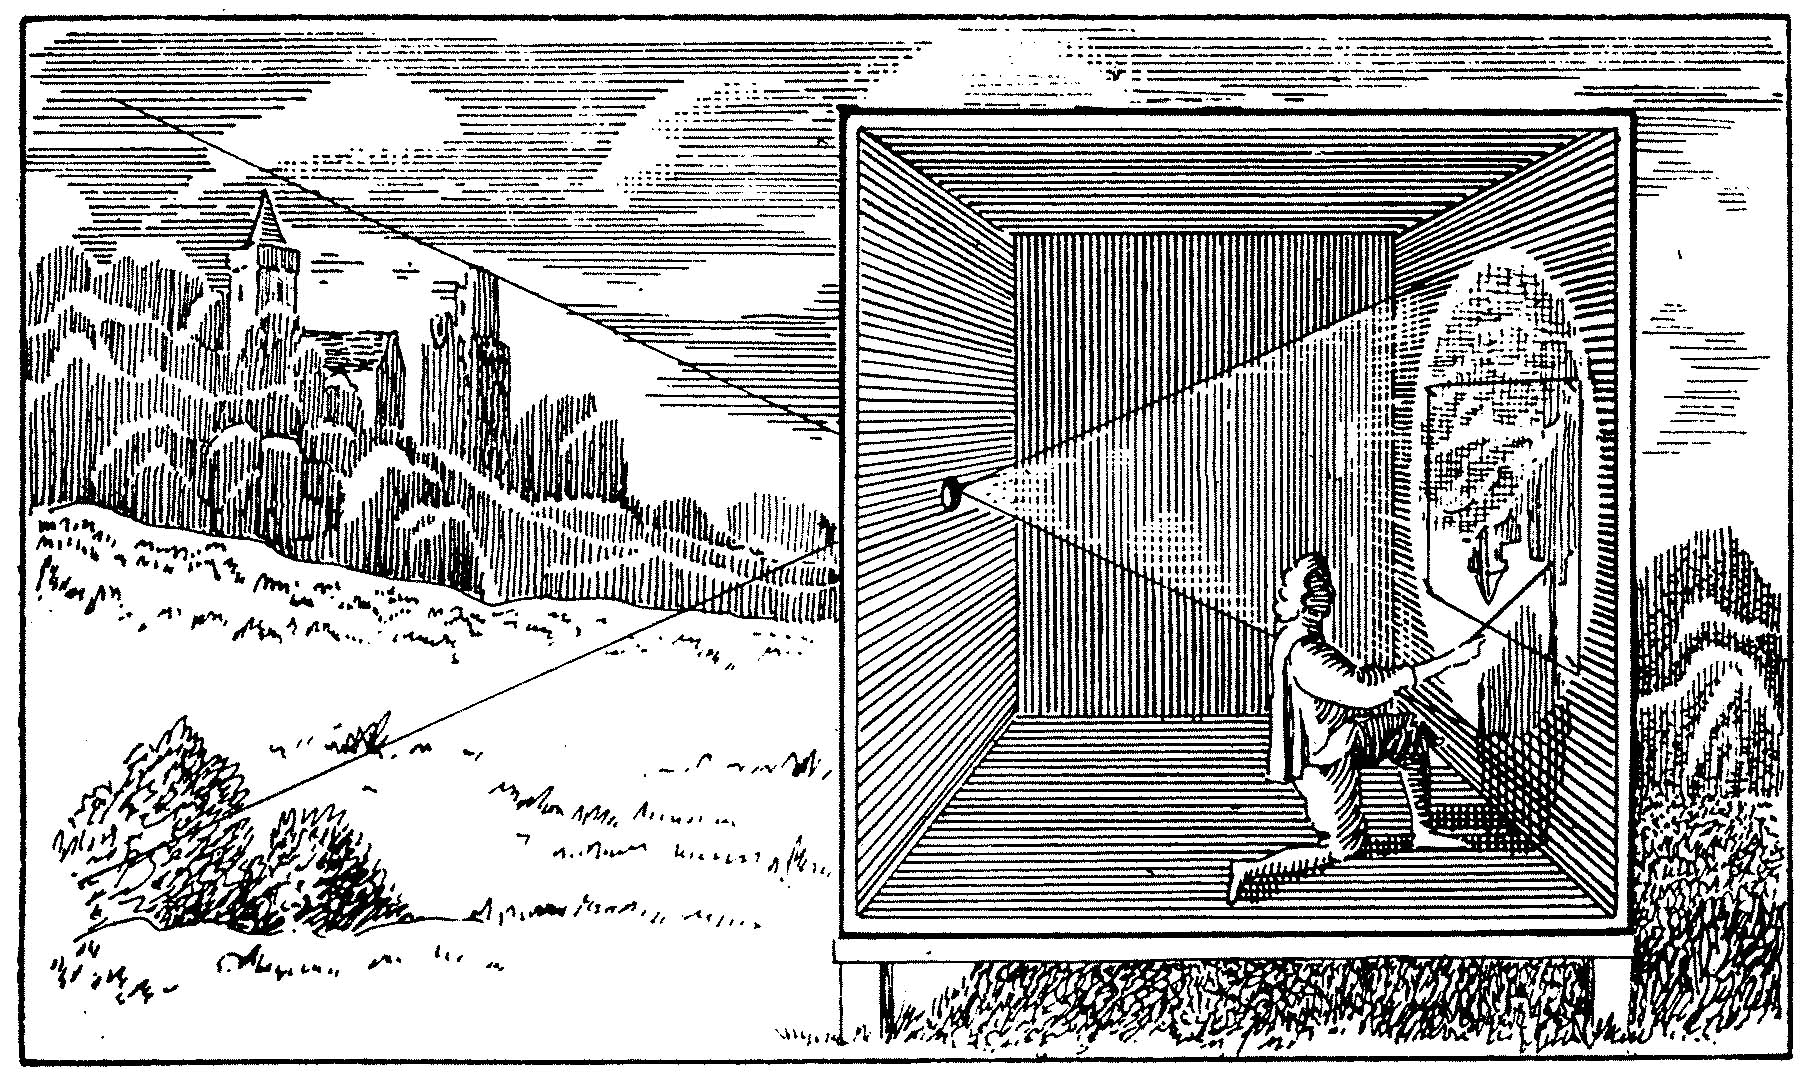
\includegraphics[width=\textwidth]{img/cameraobscura.jpeg}
\end{figure}

\vspace{8cm}
\center{Dominik Schlegel}
\center{\today}

\end{titlepage}


\newpage

\section*{Preface}

On the following pages I will discuss the development of the human perception model and its
inseparable relations to the scientific body in the 19th century. The essay focusses on
{\it{Subjective Vision and the Separation of the Senses}} \cite{crary} and includes information from
{\it{Techniques of the Observer}} \cite{crary}, {\it{The Images of Precision: Helmholtz and the
Graphical Method in Physiology}} \cite{holmes} and {\it{Camera and Mind}} \cite{ellenbogen}. Basic
knowledge of the material is assumed and only the key points will be repeated in order to explain
my view.

As an additional, diverse source I picked a topic about the beginning of the institutionalization of people
with disabilities during the 19th century and its direct connection to the respective idea of
perception and human society \cite{earlymovement}.

\section*{Thesis}

I claim that the change from the 18th centuries humanly passive and pseudo-objective
perception to the physiologically objective perception of the 19th century was crucial in order to
enable the massive growth in production of scientific knowledge during the 19th century.
The human body was far from being completely understood at the end of the 18th century but
nevertheless people took perceived impressions as the undiluted, completely clear representation of
their true nature.
This premise reduces the observer to a simple, passive receiver of information without any transformation
of the input from outside - which is not entirely true as we know nowadays.
One can easily think about the numerous possible conflicts resulting from parties with differently developed
senses (e.g. eyesight).

At the same time researches started to play around with the senses and challenged this humanly passive model
of perception. As a result people became unsure about the intake of their senses and the human body
manifested itself as the nature of perception (from physics to physiology). The human body can therefore be
seen as a black box, an object in which we do not not what is going on but in which we expect a
transformation of the input. The step to the acceptance of this black box is of prime importance to me.
Having the black box model researchers could start to quantify perception and get closer to truth
representations of nature.

Additionally one should not forget the inherent link between the new model of perception and human society.
The researchers pursuing this model of perception had many contestants and had a hard time publishing
their findings in the beginning of the physiological movement.

Relating to my second source, people whose senses were non- or malfunctional were not able to perceive nature
based on the humanly passive model - and as a consequence were not accepted by the broad human society. This
changed with the model of perception, whereas it became clear that every human transforms nature and
therefore nobody can tell the actual truth of an occurrence. I do not say that this was the major reason for
rise of the institutionalization of people with disabilities but it certainly did play its part.

\section*{Reading}

{\it{Subjective Vision and the Separation of the Senses}} is a chapter of the book {\it{Techniques of the
Observer}} \cite{crary} written by Jonathan Crary. The essay is composed upon a literature collection and
refers to various famous historical figures. The two major topics discussed are the rise of physiology and
the establishment and reframing of new sciences.

In the following sections I will cover the main aspects of the reading and relate them to my Thesis.
Since the topics sometimes overlap with sections discussed in other readings, I will include that
information and mention the respective sources.

\subsection*{The Camera Obscura and Subjective Vision}

The camera obscura is an optical device based on the principle of the pinhole camera model \cite{camera}. While
the principle has been known to mankind since approximately 400 BCE, a sufficiently precise realization of the
camera obscura was not achieved until the end of the 16th century. In the 17th century more people began to
work with the device and some started to develop theories about its relation to the human observer.

One of them was Isaac Newton who showed that a ray of white light - the portion of light passing through the
inlet of the camera obscura could be separated into the rainbow colors by using a prism \cite{newtongoethe}.
Newton published his findings in his major work: {\it{Opticks or a treatise of the reflections, refractions,
inflections andcolours of light}} \cite{opticks}.
It is important to note that the influence of physiology on perception
was not part of Newton's studies. The camera obscura established unclouded relations between
the artificial world inside the box and the natural world outside and enabled a clear separation
and definition of object and observer. The observer himself was not of interest for Newton and therefore the
possible correctness of observations was not challenged nor verified in terms of quality.

Over a hundred years later Johann Wolfgang von Goethe made the camera obscura the site of his optical studies
as well. Goethe summarises his work in the {\it{'Farbenlehre'}} \cite{farbenlehre}. 
Goethe denied and battled Newton's theories about white light. For Goethe white light was the visible
absence of color whereas for Newton white light was the sum of all colors - this is a crucial difference
with correspondingly diverse resulting theories. As we know by today Newton was right, but at that time it
was not clear which theory is correct and Goethe made important discoveries, even though he seemed to be on
the wrong path from the start.

In contrast to Newton, Goethe started to involve physiology in his optical studies. This is the point where
the question of the human black box will turn up. Goethe created the perfect scenario for displaying the
physiological effects on the sense of sight and therefore on the observer by only a minimal modification of the
camera obscura: Goethe sealed the hole after a short aperture time.

The observer could now still experience an image even thought there was no
light source present. This contradicts the logic behind an observer seeing only real objects visible to him.
The resulting shift from a constant, passive, objective observer to a physiologically active, subjective
observer defines the human body as the active producer of an optical experience and as a direct
consequence, of all sensory experiences.
Thanks to this step the existence of a black box, the human perception as an active system became
undeniable. One speciality about Goethe's observer model is the inseparability of two models usually
presented as distinct and contradictory: the observer as a strictly physiological system and the
autonomous, independent producer of his/her own experiences.

At the same time other researchers such as Immanuel Kant strengthen this change of the point of view
in vision with their discoveries. William Blakes agrees on the model and Michel Foucault
emphasizes the the inconsistent relation to the old model.

Goethe and other researchers continued working with the sense of sight and began to discover
properties of the black box.
This means that the human itself started to examine the complex properties of its perception
in form of a legion of researchers for the first time. Because of the complexity of this topic
straight and efficient progress is not expected and researchers had numerous conflicts with
their colleagues in certain fields. Even though the conflicts slowed down the derivation of a
universal model, they guaranteed the maximum variety of studies to select from.

Later on Arthur Schopenhauer came up with heavily physiological theories on the subject. Schopenhauer
abandoned the combination of the two models Goethe used for his observer. According to Schopenhauer
the experience of color could only result from physiological phenomena. Even thought they disagreed on
that specific topic, both of them were against the Newtonian optics. Schopenhauer also rejected any model
of the observer as passive receiver of sensation as described by John Locke and Étienne Bonnot de Condillac.
The notion of correspondence between subject and object disappears for Schopenhauer and he
builds the complete perceptional apparatus upon the body of the observer. For him the distinction of
interior and exterior is irrelevant since it is only a construction of the human mind.

Starting from a simple optical device, the camera obscura and intense involvement in the sense of sight
Schopenhauer ended up questioning the view of reality. Schopenhauer also contested the works of Kant
and defined 'Vorstellung' as pure physiological phenomenon and criticizes the pure philosophical nature
of Kant's work. Another figure which was of grate importance to Schopenhauer was Xavier Bichat.
He provided Schopenhauer with a crucial physical model of the human subject helping him to manifest
his theories and had the same strong physiological ideologies as Schopenhauer.

The author preserves a neutral stance over the complete section and is able to provide
very dense information in a enjoyable way. The important background knowledge about occurring
personalities is not reserved and the reader can get a deep insight into the respective events.
The focus lies primarily on Goethe and as the text advances on Schopenhauer which gives an important spice
to the covered topics. Whereas I am only concerned about the main points regarding the evolution of the
model of perception the author lists various specific developments in great detail and mentions their
influence on the subject.

I end this section with a quote from the author which, in my opinion could not have better caught
the essence of the topic:

\begin{quote}

The subjective vision affirmed by Goethe and Schopenhauer that endowed the observer with a new perceptual
autonomy also coincided with the making of the observer into a subject of new knowledge and new
techniques of power. The terrain on which these two interrelated observers emerged in the nineteenth
century was the science of physiology. 

{\it{Subjective Vision and the Separation of the Senses}} \cite{crary}, page 79 first paragraph

\end{quote}

\subsection*{The Rise of Physiology}

Keeping the quote from the previous section in mind we move on to the discussion of the
emerge of physiology as a science.
It is clear that the strongly increasing occurrence of physiological aspects in the studies of many
prestigious researches demanded a institutionalization of physiology. Even thought the involvement
of physiology began already before the 19th century it became not formally specialized before 1940.
This change signalled how the human body was becoming the center of power and truth.
Scientists explored the aspects of the human body in great depth and by 1826, Johannes Müller
determined that sensory nerves are of five types. A first quantification of the black box has been made.
At the same time Pierre Flourens was able to identify functions of the different parts of the human
brain. A discretization of the brain into cerebellum, motor center and cerebrum, a perception center,
was the result his studies.

The ongoing evolution of physiology provided Schopenhauer with sufficient amounts of information to
ground his theories and vice versa. He isolated the perceptional part from the human body and
focussed on the way how reality is created by the observer. It became clear that perception is not
uniform in all men or women and therefore the black box can not be generalized. Schopenhauers urge to
find the pure objectivity of perception was extraordinary. Another important point is that
Schopenhauer insisted on the possibility of physical methods manipulating the certain modes of
perception. Relating to his remarkable physiological description of beauty one can easily see that
a cup of water is more appealing to a thirsty hiker just returning from the desert than to a
guy swimming in a mountain spring. It is assumed that both persons appreciate a cup of water to
the same amount if they are located in the same physical environment.
The cup of water is in the same physical condition in both cases but the observer underlies different
conditions, the perception is modified by physical stimuli.

The study of the eye was also an important part of another growing new discipline: the science of
physiological psychology. Here the relation to economy becomes visible, by a quantification of
perception processes could be optimized and executed more efficiently. One example would be just the
coordination of eye and hand which is required in almost every profession. The resulting
knowledge enabled techniques for the external control of the observer, the physical methods
Schopenhauer was already aware of.

Simultaneously the wave theory of light gained on importance in the 19th century.
Thanks to Augustin Jean Fresnel's work in 1821 and various other achievements of influential figures 
during that time the wave theory became broadly accepted and made many of the large,
classical theories in optics obsolete. The rise of physiology as a science is inherently linked
to the conflicts in the other sciences. The subject of optics moved out of its well-defined box
and merged with studies of other physical phenomena.
As a result physical optics even merged with physics and physiological optics began to dominate
the study of vision itself. The study of vision or more general perception were a huge part of physiology
during that time.

One famous physiologist was Johannes Müller who published the {\it{Handbuch der Physiologie des Menschen}},
a heavily physiological work about the human organism. Müller describes the observer in a pure physical and
mechanical way and leaves out any romantic aspects. The very distinct work of Müller began quickly to have
a major influence on physiology and psychology in the mid-19th century. One famous student of Müller was
Hermann von Helmholtz, who will play an important role in the section about the graphical method later on.
Müller's theories about perception with the sense of sight as the biggest topic were the most influential
part of his work. Müller shaped the model of the observer and demonstrated for the sense of sight that
an observer could experience light in the absence of any actual light.
This again shows the possible modification of perception Schopenhauer also mentioned.
Müller examined this particular situation in great detail and enumerated five agencies capable of 
manipulation the sense of sight and producing the sensation of light.
He figured which inputs to the black box would generate always identical outputs.
The fact of possible identical results with different original situations demanded a new way of
observing. The way how scientific studies have to be done has to be adjusted to take the human
black box into account.

The findings of Müller made the camera obscura model irrelevant and confirm the subjectivity of vision.
A redefinition of vision followed and new forms of reality and the capacities of the black box were
proclaimed. As a consequence skepticism  about the unreliability of the senses came up.
Whereas for Müller perception is constituted from five isolated, distinct senses Emil Dubois-Reymond,
a colleague of Helmholtz, thought about cross-connections between the senses such as the eye seeing
sounds and the ear hearing colors. One can see how far this exploration of the black box went and
what abstract theories turned out to be true.

In an essence, Müller and other recognized researchers gave physiology the power to emerge as a
formal, independent science in the 19th century. The author elaborates heavily on Müller and relates him
to other important researchers such as his pupil Helmholtz. The author sometimes slightly shows
skepticism about certain topics persuaded by researchers, which seem far off from the track to a regular person.
As for the first part, the passage is very vivid and many different aspects are discussed in
just the right amount of detail knowledge required.

\subsection*{Magic Tricks}

Lets now move on to the reading {\it{Techniques of the Observer}} \cite{crary} which will allow us
to further explore the discovery of the black box. The discussion will not be as detailed as before
since this was not the main reading. This topic is relevant to me because it describes the invention and
integration of devices interaction with human perception, mainly the sense of sight.

Considering the camera obscura the term optical illusion shows up. For Goethe there was no such
thing as an optical illusion, whatever the healthy corporal eye experienced must be the optical truth.
This does not necessarily imply that what you see is the truth, but only that it is the optical truth.
Since the experienced optical phenomenon also changed over time it challenged the instantaneity
of optical transmission which was an ancient, broadly accepted theory.
Johann Friedrich Herbart attempted to mathematize perception and prepared the grounds for the
first objective measurements of optical events such as the afterimage.

Goethe used the term afterimage to label the optical illusion resulting from the modification of the
observed object.
The studies of the afterimages was occurring in a wide range of scientific research by the
1820s and led to various inventions of related optical devices and techniques.
Thanks to the definition and reproducibility of an afterimage it became one of the first
objects by which observation, the process containing the black box, could be quantified.
Researchers could measure elements like the intensity and duration of an afterimage and produced
scientific data containing the dependency of the observer itself.

Optical illusions became a popular form of entertainment in the 19th century and they still are today.
The inclusion of the entertainment sector allowed the researches to spread their ideas and
motivate possible newcomers. Even though people experienced optical illusions already before
physiologists started to explore their functionality, the phenomena were not given any scientific
explanations. This step was crucial for the invention of most of the optical devices we possess nowadays
and supports my claim that perception had to be quantified and applied.

\subsection*{The Graphical Method}

The graphical method is a procedure described by Helmholtz in 1847 which was substantial for later
experiments in physiology. This topic originates from the text {\it{The Images of Precision: Helmholtz
and the Graphical Method in Physiology}} \cite{holmes} and I include it in my essay because
it nicely displays how people reacted to this method based on the notion of perception.
Additionally the emerge of the graph as a representation of scientific data will be briefly discussed.

Helmholtz participated in the movement of chemistry as well as physics and his experimental
procedures substantiated general quantification and precision measurement in the 19th century.
The definition of such tools is crucial in order to produce objective science and keep the
maximum potential for further interpretation of scientific data.
At the same time the black box is inseparable from the observer and researchers had to
think about tools which provided true representations independent from the observer.
This task was more challenging than one might think.

The difficulties in finding an optimum description of a process can be seen by reference to
Helmholtz's graphical method. Helmholtz first intended to measure the time-course of
muscle contractions and not the timings of the nerve impulse.
The fact that he changed the property to measure shows us that he found a better
representation of the phenomenon than the original one. Helmholtz never returned explicitly to
the original representation. In the end the graphical method described a procedure
capable of the autonomous drawing of muscular behaviour. The enormous popularity of
the graphical method helped experimental physiology the emerge during the 1840s
and marked the beginning of the application of mathematical analysis to physiological
phenomena. The popularity of the method did not necessarily imply its undeniable acceptance among
other researchers. The question of true representation and the choice of the best measurements
became intensely discussed in scientific circles.

The value of the graph as a representative tool became indubitable. Leonhard Euler wrote the first
paper about graph theory in 1736 \cite{graphtheory} but the graph did not gain popularity until the middle of
the 19th century thanks to the physiologists and the ongoing industrialisation.
The graphical method of Helmholtz introduced a self-drawing graph. The term self-drawing is 
of immense importance since it means that the observer gets completely excluded from the creation
of a representation of the phenomenon. For physiologists the self-drawing graph was the purest form
of information since it was not influenced by the human black box and therefore must be truly objective.
Helmholtz struggled with his own achievement as he developed a second method being more precise than
the first one but required the observer to draw the graph from numerical data.
Having the observer involved it the ideal representation was no longer guaranteed but Helmholtz managed
to combine his methods and published a document in which he showed that both of them are
similarly correct. Many other researcher were conducting studies on muscle behaviour as well independently
of Helmholtz. One of them was Alfred Volkmann who represented his observations completely in numerical
tables. Volkmann did not draw graphs from his data but applied mathematical principles to
his idea of the true form of the graph and draw those. Both ways of representation, the graphical and
the numerical one turned out to be great tools for the display of scientific data and one could not
imagine today's world without them.

In addition to the discovery of these tools one should not forget the possibility of measuring
events which can not be caught by the human observer became available thanks to the invention of
machines like Helmholtz used for the graphical method. The belief in information which the
human perception can not retrieve by itself is crucial for the evolution of science.
The level of abstraction kept increasing over the years and amazing concepts could be derived
(e.g. Higgs boson, the God particle)

\subsection*{Flying Horses}

Going one step further in the representation of scientific truth I want to talk about a
tool which revolutionized the scientific world. In the essay {\it{Camera and Mind}} \cite{ellenbogen} Josh
Ellenbogen describes how the photograph started to replace the experiment itself.

Camera photography came up in the first decades of the 19th century and continuously gained scientific
popularity in the 1830s. The power of the tool was immense, similar to the graphical method researchers 
could now observe phenomena invisible to the human eye. The motion of the human body became the
center of attention for most studies and elementary principles were discovered.

As for the graphical method the camera is a mechanized, self-writing device and its functionality is
completely detached from the observer. The camera could be seen as an agent of knowledge or scientific
truth as Ellenbogen states. In a sense the camera replaced the observer completely.
The belief in photography was controversial in the 19th century.
Photographs could easily be manipulated and mediate wrong representations of the truth.
Researchers modified their subjects and transformed the resulting photographs further into regular
graphs to gain a clear visualization of the experiment. The idea of objectivity has to be
reconsidered and the trust in abstraction grew as photography was applied to more fields of society.

Photography became applied to sectors other than science such as law. By capturing images of criminals
and distribution among the other departments they could get easily recognized.
Photography extended the observers functionality by creating permanent memory and genuine information
exchange. The power of photography can also be seen by a dispute in the science of art in the 19th
century. By taking pictures from a galloping horse researchers found out that at some point all legs
of the horse are completely off the ground. Artists however draw horses since ages always with one foot
on the ground in their paintings. As the information passed through some started to draw flying horses with
all their feet up in the air while others kept the original model.

The discussion of reality is more complex for art. It is not clear whether the representation of the truth
for a painting is what the human eye can see or what the human mind can create.

\section*{Conclusion}

The different readings tell the story of the emerge of physiology as a science and the exploration of reality
by researchers of the 19th century. Based on the respective historical events I see my claim
proofed that the observer had to become aware of the black box and challenge reality in order to
produce promising scientific knowledge. The beginning with the camera obscura and the
resulting redundancy of itself shows me the massive ideological change researchers were able to grasp.
With their studies about optical illusions, the graphical method and photography physiologists could apply
their models of the observer and smooth the way for industrialisation.

\newpage

\bibliographystyle{unsrt}
\bibliography{references.bib}

\end{document}
